\documentclass[../DS04.tex]{subfiles}
\graphicspath{{./figures/}}

% \subimport{/home/nora/Documents/Enseignement/Prepa/bpep/exercices/DS/resonance_verre/}{sujet.tex}

\begin{document}

\section[86]"P"{Résonance d'un verre\ifcorrige{~\small\textit{(D'après TSI Centrale
		Supélec 2018)}}}

\enonce{%
Dans le vingt-et-unième album de la série {\it Les Aventures de Tintin},
intitulé {\it Les Bijoux de la Castafiore}, cette dernière est en mesure de
faire exploser un verre par la simple utilisation de sa voix. Le présent sujet
se penche sur les aspects physiques de ce phénomène. Nous tenterons ainsi de
déterminer les circonstances dans lesquelles il est effectivement possible de
réaliser une telle prouesse et nous nous pencherons sur les rôles joués par les
différents paramètres physiques susceptibles d'influer sur ces circonstances.
\bigbreak
\begin{center}
	\textbf{Les deux parties sont indépendantes}.
\end{center}
}

\subsection{Analyse expérimentale des vibrations du verre suite à un choc}

\enonce{%
	Il est extrêmement facile, en frappant un verre à pied, d'entendre le son que
	celui-ci émet. On se propose dans cette partie de déterminer, à partir d'une
	modélisation simple, quelques propriétés des oscillations libres d'un verre
	mis ainsi en vibration.
	\begin{center}
		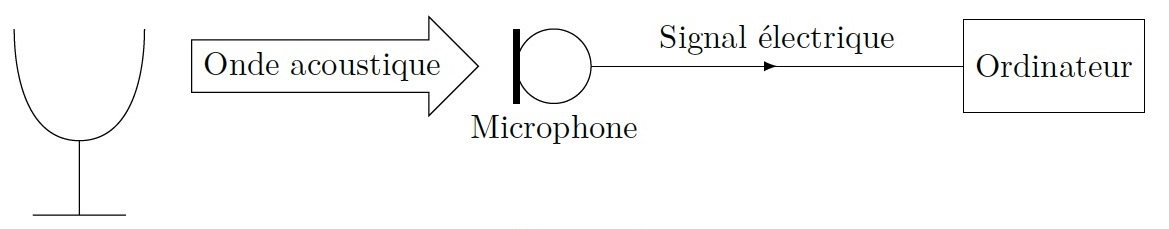
\includegraphics[width=.6\linewidth]{res_verre_1}
		\vspace{-15pt}
		\captionof{figure}{Schéma de principe.}
		\label{fig:schema_principe}
	\end{center}
	Un verre à pied, d'un diamètre de \SI{12}{cm}, est frappé, à l'instant $t=0$,
	au niveau du bord supérieur à l'aide d'un petit marteau. Le son émis est
	enregistré par ordinateur et représenté sur la figure \ref{fig:chronogramme}.
	Le spectre de ce signal temporel est représenté sur la figure
	\ref{fig:spectre}.
	\smallbreak
	\noindent
	\begin{minipage}[c]{.42\linewidth}
		\begin{center}
			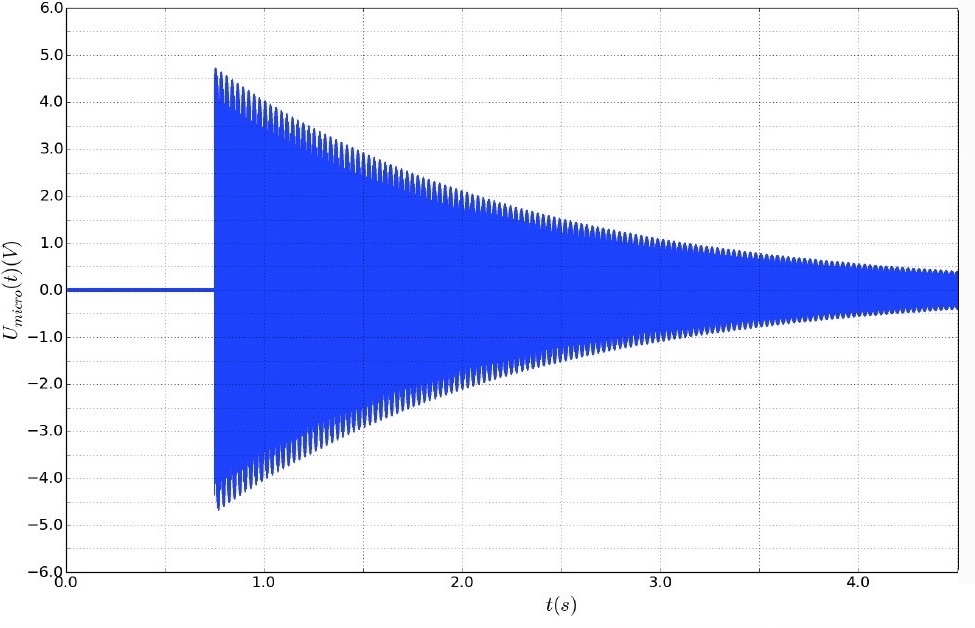
\includegraphics[width=\linewidth]{res_verre_2}
			\captionof{figure}{Chronogramme de l'enregistrement sonore du verre.}
			\label{fig:chronogramme}
		\end{center}
	\end{minipage}
	\hfill
	\begin{minipage}[c]{.5\linewidth}
		\begin{center}
			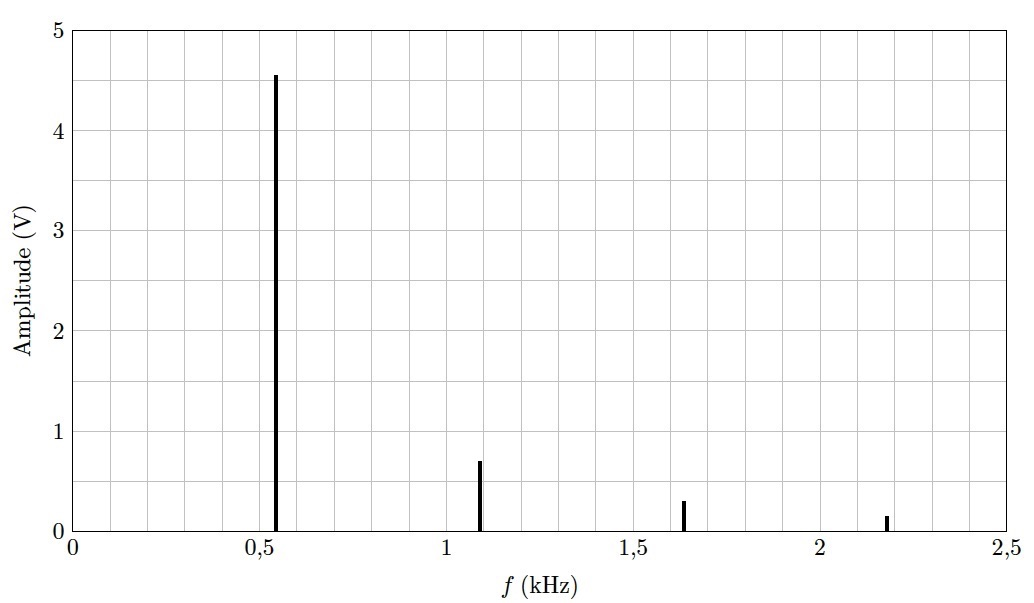
\includegraphics[width=\linewidth]{res_verre_3}
			\captionof{figure}{Analyse spectrale du son réalisé peu après la frappe du
				verre.}
			\label{fig:spectre}
		\end{center}
	\end{minipage}
	\bigbreak
	Les «~pics~» représentés dans la figure \ref{fig:spectre} correspondent à des
	modes propres de vibration du verre.
}

\QR[5]{%
	Donner les fréquences des différents modes propres. Elles sont liées par une
	relation simple, laquelle~?
	Comment nomme-t-on ces différents modes propres~?
	Quelle est la fréquence du signal~?
}{%
	On relève les fréquences suivantes~: $f_1\approx \SI{550}{Hz}$, $f_2\approx
		\SI{1090}{Hz}$, $f_3\approx \SI{1620}{Hz}$ et $f_4\approx \SI{2180}{Hz}$.
	\pt{1} On remarque donc que l'on a $\boxed{f_n= n f_1}$, avec $n\in
		\mathbb{N}^*$ \pt{1}
	\smallbreak
	Le premier mode est appelé \xul{fondamental}. \pt{1} Les autres sont appelés
	\xul{harmoniques de rang $n$}. \pt{1}
	\smallbreak
	La fréquence du signal est la fréquence de son fondamental, donc ici
	\xul{$f=\SI{550}{Hz}$.} \pt{1}
}

% \QR{%
%   À l'aide d'un modèle simple, que vous exposerez clairement, déterminer la
%   vitesse de propagation de l'onde de choc dans le verre. \textit{Cette question
%   nécessite de prendre des initiatives. Il n'est pas nécessaire d'y avoir
% répondu pour poursuivre le problème. La notation portera sur l'ensemble de la
% démarche mise en place (identification des phénomènes physiques intervenant,
% hypothèses simplificatrices, etc) et non pas sur le seul résultat.}
% }{%
%   La présence de plusieurs modes propre indique qu'on est en présence d'ondes
%   stationnaires de même type que celles de la corde de \bsc{Melde}.
%
%   Or, le mode fondamental de la corde de \bsc{Melde} se caractérise par une
%   fréquence fondamentale $f_0=\frac{c}{\lambda}$ avec $\lambda=2L$. La longueur
%   d'onde est donc égale à la distance parcourue par l'onde pour revenir au point
%   où elle a été émise. En effet, on peut aussi voir le problème en terme
%   d'interférences : quand l'onde réfléchie atteint le vibreur, elle a parcourue
%   une longueur d'onde et se trouve donc en phase avec l'onde émise par le
%   vibreur, ce qui crée des interférences constructives entre les deux ondes, et
%   donc un mode de résonance.
%
%   Dans le cas de l'onde de choc se propageant dans le verre, on peut considérer,
%   pour simplifier le problème ici que l'onde se propage en suivant le bord du
%   verre. Sur le même principe que la corde de \bsc{Melde}, la longueur d'onde du
%   mode fondamental doit donc être égale à la distance parcourue par l'onde avant
%   de revenir à son point de départ, soit $\lambda=2\pi R=\pi D$. On a alors
%   $c=\lambda f$. L'application numérique donne $c=\pi \times 0,12 \times 540
%   \approx \SI{2,0e2}{m.s^{-1}}$.
% }

% \vspace{0.5cm}
\enonce{%
	Quand le verre est en vibration, son bord supérieur oscille autour de sa
	position au repos. Afin d'estimer le facteur de qualité du verre, on le
	modélise par une masse $m$ mobile sur l'axe $(Ox)$ horizontal associée à un
	ressort de raideur $k$, de longueur à vide nulle (figure
	\ref{fig:schema_mecanique_verre}). Les frottements seront, quant à eux,
	modélisés par un frottement fluide de type $\vv{f} = - \alpha \vf$ où $\vf$
	désigne le vecteur vitesse de la masse $m$.
	\smallbreak
	\noindent
	\begin{minipage}[c]{\linewidth}
		\begin{center}
			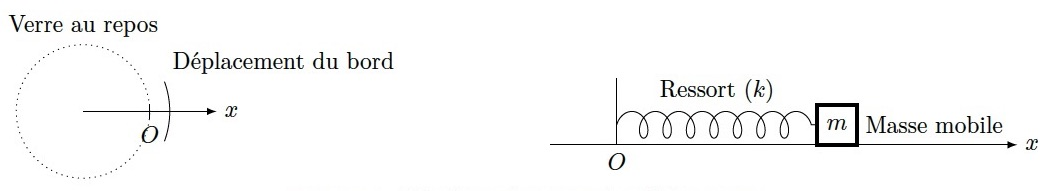
\includegraphics[width=.8\linewidth]{res_verre_4}
			\captionof{figure}{Modèle mécanique du déplacement.}
			\vspace{-15pt}
			\label{fig:schema_mecanique_verre}
		\end{center}
	\end{minipage}
}

\QR[10]{%
	Établir proprement le système d'étude.
}{%
	\pt{2} pour un beau schéma propre.
	\smallbreak
	\noindent
	\begin{isd}
		\begin{itemize}
			\item[l][15]{\pt{1}} Système~:
			      \{point M\} de masse $m$
			\item[l][15]{\pt{1}} Référentiel d'étude~:
			      $\Rc\ind{sol}$ supposé galiléen
			\item[l][15]{\pt{1}} Repère~:
			      $(\Or, \ux, \uy)$ avec $\uy$ vertical ascendant
			\item[l][15]{\pt{1}} Repérage~:
			      $\vv{\rm OM} = x(t)\ux~;
				      \vf = \xp(t)\ux~;
				      \af = \xpp(t)\ux$
		\end{itemize}
		\tcblower
		\begin{itemize}
			\item[b]{Bilan des forces~:}
			      \[
				      \begin{array}{ll}
					      \pt{1} \textbf{Poids}            &
					      \Pf = m\gf = -mg \uy
					      \\
					      \pt{1} \textbf{Réaction support} &
					      \Rf = R\uy
					      \\
					      \pt{1} \textbf{Force rappel}     &
					      \Ff = -k(\ell(t) - \underbracket[1pt]{\ell_0}_{=0}) \ux =
					      -k x (t) \ux
					      \\
					      \pt{1} \textbf{Force frottement} &
					      \Ff_{\rm frott} = -\alpha\vf = -\alpha \dv{x}{t} \ux
				      \end{array}
			      \]
		\end{itemize}
	\end{isd}
	\vspace{-15pt}
}%

\QR[5]{%
Montrer que l'équation différentielle traduisant l'évolution temporelle de
$x(t)$ s'écrit de la façon suivante, avec $\w_0$ et $Q$ deux constantes que
l'on exprimera en fonction de $\alpha$, $k$ et $m$~:
\[
	\dv[2]{x}{t} + {\frac{\w_0}{Q}}{\dv{x}{t}} + \w_0^2 x = 0
\]
}{%
~
\vspace{-15pt}
\smallbreak
\noindent
\begin{isd}[interior hidden]
	Avec le PFD~:
	\begin{DispWithArrows*}[groups]
		m\af & \stm{=} \Pf + \vv{R} + \Ff_f + \Ff_r
		\CArrow{$\cdot \ux$}
		\\\Ra
		m \dv[2]{x}{t} + \alpha \dv{x}{t} + k x(t) & = 0
		\CArrow{$\mdiv m$}
		\\\Lra
		\dv[2]{x}{t} +
		\frac{\alpha}{m} \dv{x}{t} +
		\frac{k}{m} x(t)                                 & \stm{=} 0
	\end{DispWithArrows*}
	\tcblower
	On identifie $\w_0$ et $Q$~:
	\begin{gather*}
		\w_0{}^2 = \frac{k}{m}
		\Lra
		\boxed{\w_0 \stm{=} \sqrt{\frac{k}{m}}}
		\\\beforetext{et}
		\frac{\alpha}{m} \stm{=} \frac{\w_0}{Q}
		\Lra
		Q = \frac{m\w_0}{\alpha}
		\Lra
		\boxed{Q \stm{=} \frac{\sqrt{km}}{\alpha}}
	\end{gather*}
\end{isd}
D'où la forme demandée.
}

\QR[3]{%
	Quels sont les noms, les unités et les significations physiques de $\w_0$ et
	de $Q$~?
}{%
	$\w_0$ est la pulsation propre \pt{0.5} du système, elle s'exprime en \si{rad/s}
	\pt{0.5}. Elle correspond à la pulsation à laquelle oscillerait le système s'il
	n'y avait pas de frottement. \pt{0.5}
	\smallbreak
	$Q$ est appelé facteur de qualité du système. \pt{0.5} Il est sans unité.
	\pt{0.5} Plus $Q$ est grand, moins il y a de dissipation d'énergie, plus le
	système s'approche d'un oscillateur harmonique non amorti. \pt{0.5}
}

\QR[9]{%
	Compte tenu du choc initial avec le marteau, déterminer, dans le cas de
	frottements «~faibles~», l'expression approchée de la solution $x(t)$. Montrer
	en particulier que la fonction $x(t)$ peut se mettre sous la forme d'un signal
	sinusoïdal de pulsation $\W$ délimité par une enveloppe exponentielle
	décroissante, dont on précisera l'expression du temps caractéristique $\tau$
	en fonction de $\w_0$ et $Q$.
}{%
	L'équation différentielle est homogène, donc $x(t)=x_h(t)$. \pt{1} Pour
	déterminer $x_h(t)$, on injecte la forme générique $x_h(t) = K \exr^{rt}$
	\pt{1} pour trouver l'équation caractéristique~:
	\smallbreak
	\noindent
	\begin{isd}
		\begin{DispWithArrows*}[fleqn, mathindent=-10pt, groups]
			r^2 + \frac{\w_0}{Q} r+ \w_0^2 &\stm{=} 0
			\\\Ra
			\Delta &\stm{=} \frac{\w_0{}^{2}}{Q^{2}}\left( 1-4Q^{2} \right) \stm{<} 0
			\makebox[0pt][l]{\quad \text{faible amortissement}}
			\\\Ra
			r_\pm & \stm{=} \frac{-\frac{\w_0}{Q} \pm \jj\sqrt{-\D}}{2}
			\Arrow{On injecte $\Delta$}
			\\\Lra
			r_\pm &= -\frac{\w_0}{2Q} \pm
			\frac{\jj}{2} \sqrt{\frac{\w_0{}^{2}}{Q^{2}}\left( 4Q^{2}-1 \right)}
		\end{DispWithArrows*}
		\tcblower
		\begin{DispWithArrows*}[groups]
			\Lra
			r_\pm &\stm{=} - \frac{\w_0}{2Q} \pm \jj \frac{\w_0}{2Q} \sqrt{4Q^{2}-1}
			\Arrow{$\W$ et $\tau$}
			\\\Lra
			r_\pm &\stm{=} - \frac{1}{\tau} \pm \jj\W
			\\\Ra
			\boxed{\tau=\frac{2Q}{\w_0}}
			\quad & \stm{\text{et}} \quad
			\boxed{\W=\frac{\w_0}{2Q}\sqrt{4Q^2-1}}
			\\\Ra
			\Aboxed{x(t) &\stm{=} \exr^{-t/\tau} \pa{A \cos(\Wt) + B \sin(\Wt)}}
		\end{DispWithArrows*}
	\end{isd}
	\vspace{-15pt}
}

\QR[4]{%
	Déterminer l'expression complète de $x(t)$ avec les
	conditions initiales $x(0) = 0$ et $\dv{x}{t}(0) = V_0$.
}{%
	~
	\vspace{-15pt}
	\smallbreak
	\begin{isd}[interior hidden]
		\begin{itemize}
			\item On trouve $A$ avec la première condition initiale~:
			      \begin{gather*}
				      x(0) = 0 = 1 \left[ A \cdot 1 + B \cdot 0 \right] = A
				      \quad \Ra \quad
				      \boxed{A = 0} \pt{1}
			      \end{gather*}
		\end{itemize}
		\tcblower
		\begin{itemize}
			\item On trouve $B$ avec la seconde CI~:
			      \begin{gather*}
				      \dv{x}{t} \stm{=}
				      -\frac{1}{\tau}\exr^{-t/\tau} B\sin(\Wt)  +
				      \exr^{-t/\tau} B\W\cos(\Wt)
				      \\\Ra
				      \qty(\dv{x}{t})_0 = \W B = V_0
				      \Lra
				      \boxed{B = \frac{V_0}{\W}} \pt{1}
			      \end{gather*}
		\end{itemize}
	\end{isd}
	\vspace{-15pt}
	\begin{gather*}
		\beforetext{Finalement,}
		\boxed{x(t) \stm{=} \frac{V_0}{\W}\exr^{-t/\tau}\sin(\Wt)}
	\end{gather*}
}%


\QR[4]{%
	À l'aide de la figure \ref{fig:chronogramme}, que vous recopierez sommairement
	sur votre copie pour montrer votre construction graphique, déterminer
	numériquement $\tau$.
}{%
	~
	\vspace{-15pt}
	\smallbreak
	\begin{isd}[interior hidden]
		\begin{center}
			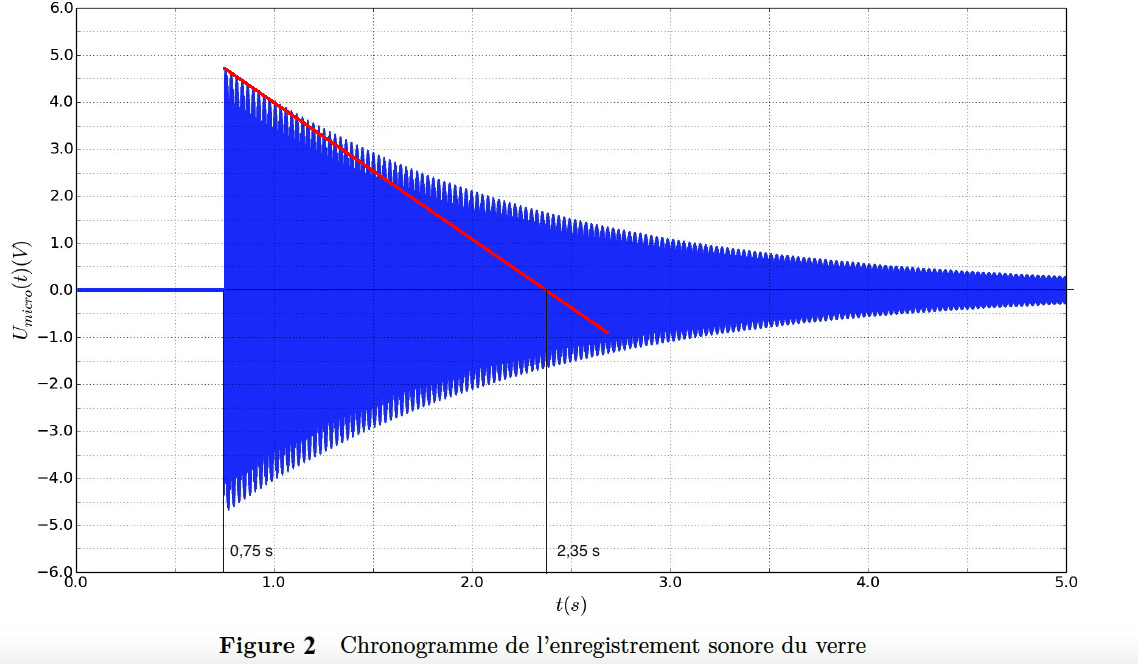
\includegraphics[width=.8\linewidth]{res_verre_2c}
			\captionof{figure}{\protect\pt{1}+\protect\pt{1}}
		\end{center}
		\tcblower
		On trace la tangente à l'origine de l'enveloppe exponentielle. Elle coupe
		l'asymptote $x=0$ en $t=\tau$. On lit donc
		\[
			\tau \stm{=} t\ind{its} - t\ind{0}
			\Ra
			\xul{\tau \stm{=} \SI{1.6}{s}}
		\]
		En effet, sur le graphique, l'excitation a lieu à $t_0=\SI{0.75}{s}$ et non
		$t=0$ comme dans la résolution mathématique.
	\end{isd}
	\vspace{-15pt}
}

\QR[2]{%
	Comment se simplifie l'expression de la pseudo-pulsation $\W$ avec l'hypothèse
	des faibles frottements (justifier précisément)~?
}{%
	On a déjà vu lors de la résolution de l'équation que
	$\boxed{\W=\frac{\w_0}{2Q}\sqrt{4Q^2-1}}$. Or, on remarque que de très
	nombreuses pseudo-périodes sont visibles, on a donc $Q\gg 1$. \pt{1} Ainsi,
	\[
		\W \approx \frac{\w_0}{2Q}\sqrt{4Q^2-\cancel{1}}
		\Ra
		\boxed{\W \stm{\approx} \w_0}
	\]
}

\QR[5]{%
	Déduire des questions précédentes les valeurs numériques de $\w_0$ et $Q$.
	Commenter le résultat.
}{%
	On a relevé précédemment la fréquence du signal $f=\SI{550}{Hz}$. \pt{1} Comme
	on a montré que $\W\approx \w_0$, on en déduit
	\begin{gather*}
		\boxed{\w_0 \stm{=} 2\pi f_0}
		\Ra
		\xul{\w_0 \stm{\approx} \SI{3,5e3}{ rad.s^{-1}}}
		\\\beforetext{De plus,}
		\tau = \frac{2Q}{\w_0}
		\Lra
		\boxed{Q \stm{=} \pi f_0 \tau}
		\Ra
		\xul{Q \stm{\approx} \num{2.8e3}}
	\end{gather*}
}

\subsection{Étude de la résonance en amplitude du verre en régime sinusoïdal forcé}

\enonce{%
On souhaite étudier plus finement la réponse en amplitude du verre au voisinage
de la fréquence de résonance du mode 1 précédemment déterminée.
\smallbreak
Un haut-parleur relié à un générateur basse fréquence produit une onde sonore
sinusoïdale de fréquence $f$. Le verre, placé à proximité du haut-parleur
(figure \ref{fig:excitation_verre}), est ainsi placé en régime
sinusoïdal forcé.
\begin{center}
	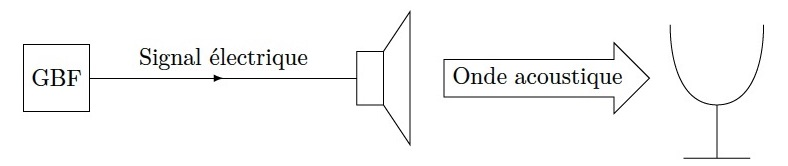
\includegraphics[width=.5\linewidth]{res_verre_5}
	\captionof{figure}{}
	\label{fig:excitation_verre}
\end{center}
L'équation différentielle traduisant l'évolution temporelle de $x(t)$ est alors
de la forme suivante, avec $\w = 2\pi f$ la pulsation et $\Phi$ la phase du
signal acoustique délivré par le générateur basse fréquence~:
\[
	\dv[2]{x}{t} + {\frac{\w_0}{Q}} \dv{x}{t} + \w_0^2 x= A_0 \cos(\w t + \Phi)
\]
En régime sinusoïdal forcé, la solution est de la forme $x(t) = X\cos(\w t +
	\f)$. On introduit la grandeur complexe associée $\xu(t) = \Xu \exp(\jw t)$
avec $\jj^2 = -1$.
}

\QR[4]{%
	Expliquer pourquoi on cherche une solution de cette forme.
}{%
	Cette équation différentielle se résout en prenant la somme de $x_h(t)$ et
	d'une solution particulière $x_p(t)$ \pt{1}. Or, on a montré dans la partie
	précédente que $\lim_{t \to \infty} x_h(t) = 0$ \pt{1}. Ainsi, en régime permanent,
	il ne reste que $x(t) = x_p(t)$.
	\smallbreak
	Or, l'entrée étant sinusoïdale, il paraît
	naturel de chercher une sortie sinusoïdale. \pt{1} De plus, l'équation différentielle
	étant linéaire, on s'attend à ce que la pulsation du signal de sortie soit la
	même que celle du signal d'entrée, sans non-linéarités. \pt{1}
}%

\QR[2]{%
Comment nomme-t-on la grandeur $\Xu$~? Que représente son module, son argument~?
}{%
$\Xu$ est appelée \xul{amplitude complexe} associée à $x(t)$. \pt{1}
$\Xu=Xe^{\jj \f}$, on a donc $\boxed{\abs{\Xu}=X}$ et $\boxed{\arg{\Xu}=\f}$.
\pt{1}
}

\QR[4]{%
	Établir l'expression de $\Xu$ puis de son module en fonction de $A_0$, $\Phi$,
	$Q$ et $u = \w/\w_0$.
}{%
	On réécrit l'équation différentielle en complexes~:
	\smallbreak
	\noindent
	\begin{isd}
		\begin{DispWithArrows*}
			\pa{(\jw)^2 + \frac{\w_0}{Q}\jw + \w_0{}^2}\Xu &\stm{=}
			\xul{A} = A\exr^{\jj \phi}
			\CArrow{$\mdiv \w_0{}^2$}
			\\\Lra
			\pa{-\pa{\frac{\w}{\w_0}}^2 + \jj \frac{\w}{\w_0Q} + 1}\Xu &\stm{=}
			\frac{A_0}{\w_0{}^2}
		\end{DispWithArrows*}
		\tcblower
		\begin{DispWithArrows*}[fleqn, mathindent=10pt]
			\Lra
			\Aboxed{\Xu(u) &\stm{=} \frac{A_0\exr^{\jj \phi}/\w_0{}^2}{1 - u^2 + \jj
					\frac{u}{Q}}}
			\Arrow{$X(u) = \abs{\Xu}$}
			\\\Ra
			\Aboxed{X(u) &\stm{=} \frac{A_0/\w_0{}^2}{\sqrt{\pa{1-u^2}^2 +
						\pa{\frac{u}{Q}}^2}}}
		\end{DispWithArrows*}
	\end{isd}
	\vspace{-15pt}
}

\QR[3]{%
	À partir d'une étude qualitative mais précise, justifier le numéro de graphe de
	la figure \ref{fig:bodes} compatible avec le tracé du module de $\Xu$ en
	fonction de la pulsation $\w$.
}{%
	On fait une étude en hautes et basses fréquences~:
	\smallbreak
	\noindent
	\begin{isd}
		\tcbsubtitle{\fatbox{\textbf{Basses fréquences}}}
		\[
			X(u) \opto{\pt{1}}{u \to 0} \frac{A_0}{\w_0{}^2} \neq 0
		\]
		\tcblower
		\tcbsubtitle{\fatbox{\textbf{Hautes fréquences}}}
		\[
			X(u) \opto{\pt{1}}{u \to \infty} 0
		\]
	\end{isd}
	On en déduit donc qu'il s'agit du \xul{graphe 2}. \pt{1}
}

\enonce{%
	\begin{center}
		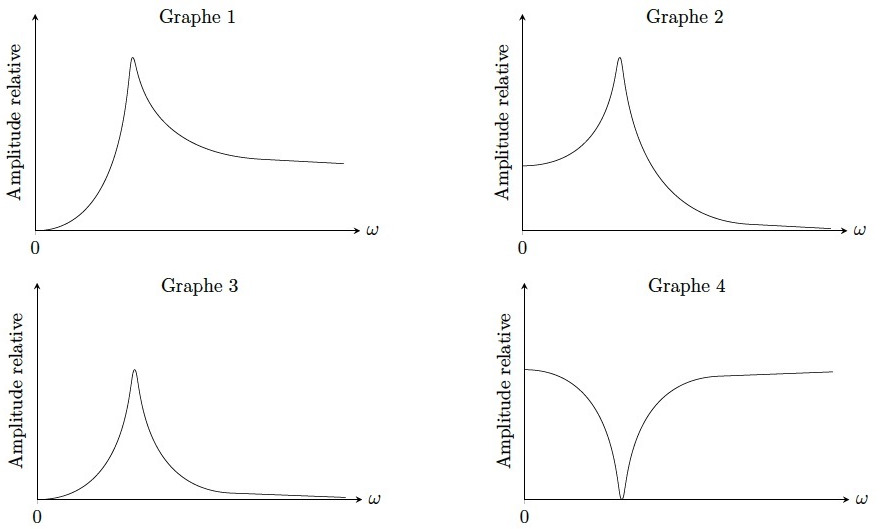
\includegraphics[width=0.7\linewidth]{res_verre_6}
		\captionof{figure}{Module de $\Xu$ en fonction de $\w$.}
		\label{fig:bodes}
	\end{center}
}

\QR[10]{%
	Montrer qu'il ne peut y avoir de résonance que si $Q>Q\ind{lim}$ et déterminer
	$Q\ind{lim}$. Donner alors l'expression de la pulsation $\w_r$ correspondant à
	la résonance.
}{%
	Pour qu'il y ait résonance, il faut que $\abs{\Xu} = X$ passe par un
	maximum \pt{1} pour $u\neq 0$ \pt{1}. Or, le numérateur de $X(u)$ est constant
	\pt{1} et la fonction racine carrée monotone donc $X$ passe par un maximum si
	la fonction $f(u)=(1-u^2)^2+\frac{u^2}{Q^2}$ passe par un minimum. \pt{1} On
	cherche donc $u_r$ tel que la dérivée de $f(u)$ s'annule~:
	\smallbreak
	\noindent
	\begin{isd}
		\vspace{-15pt}
		\begin{gather*}
			\qty(\dv{f}{u})_{u_r} \stm{=} 0
			\\\Lra
			2(-2u_r)(1-u_r^2)+\frac{2u_r}{Q} \stm{=} 0
			\\\Lra
			2u_r \pa{-2(1-u_r^2)+\frac{1}{Q^2}} \stm{=} 0
			\\\Lra
			\underbracket[1pt]{u_r = 0}_{\mathclap{\text{impossible par définition}}}
			\quad \text{ou} \quad
			-2(1-u_r^2)+\frac{1}{Q^2} = 0
		\end{gather*}
		\tcblower
		\vspace{-15pt}
		\begin{gather*}
			\Ra
			u_r^2 = 1 - \frac{1}{2Q^2}
			\Lra
			u_r \stm{=} \sqrt{1 - \frac{1}{2Q^2}}
			\\\beforetext{Possible que si}
			1 - \frac{1}{2Q^2} > 0
			\\\Lra
			Q > \boxed{\frac{1}{\sqrt{2}} \stm{=} Q\ind{lim}}
			\\\beforetext{On a alors}
			\boxed{%
				\w_r \stm{=} \w_0 \sqrt{1-\frac{1}{2Q^2}}
			}
		\end{gather*}
	\end{isd}
	\vspace{-15pt}
}

\enonce{%
	Dans la suite, on suppose $Q \gg Q\ind{lim}$.
}

\QR[2]{%
	Comment se simplifie alors l'expression de la pulsation de résonance $\w_r$ ?
	On note $X_r$ le module de $\Xu$ pour $\w = \w_r$. Établir son expression en
	fonction de $\w_0$, $A_0$ et $Q$.
}{%
	Si $Q\gg Q\ind{lim}$, alors $Q\gg 1$, et on a $\boxed{\w_r=\w_0
			\sqrt{1-\cancel{\dfrac{1}{2Q^2}}}\stm{\approx} \w_0}$
	\smallbreak
	Par définition $X_r = X(\w_r)$. D'après la question précédente, on a donc
	$X_r \approx X(\w_0)=X(u=1)$, ce qui donne
	\[
		X_r = \dfrac{A_0/\w_0^2}{\sqrt{\frac{1}{Q^2}}}
		\Lra
		\boxed{X_r \stm{=} Q\dfrac{A_0}{\w_0^2}}
	\]
}

\QR[2]{%
	Quelles sont les définitions des pulsations de coupure $\w_1$ et $\w_2$ ($\w_1
		< \w_2$) du module de $\Xu$~? On ne cherchera pas ici à établir leurs
	expressions.
	\smallbreak
	Quelle relation existe-t-il entre $\w_0$,~$Q$ et $\Delta\w = \w_2 - \w_1$ ?
	\textit{On admettra que cette relation est la même que dans le cas d'une
		résonance de type «~passe-bande~» et on cherchera pas à la démontrer.}
}{%
	Les pulsations de coupures sont définies par
	$\boxed{X(\w_1)=X(\w_2)=\frac{X_r}{\sqrt{2}}}$ \pt{1}
	\smallbreak
	L'acuité de la résonance est égale à $Q$, soit $\boxed{\dfrac{\w_0}{\Delta
				\w}=Q}$ \pt{1}
}

\enonce{%
	Une série de mesures de l'amplitude $X$ au voisinage de la résonance (réalisée
	par un dispositif interférentiel non présenté ici) permet de tracer le graphe
	représenté sur la figure \ref{fig:bode_expe}.
	\begin{center}
		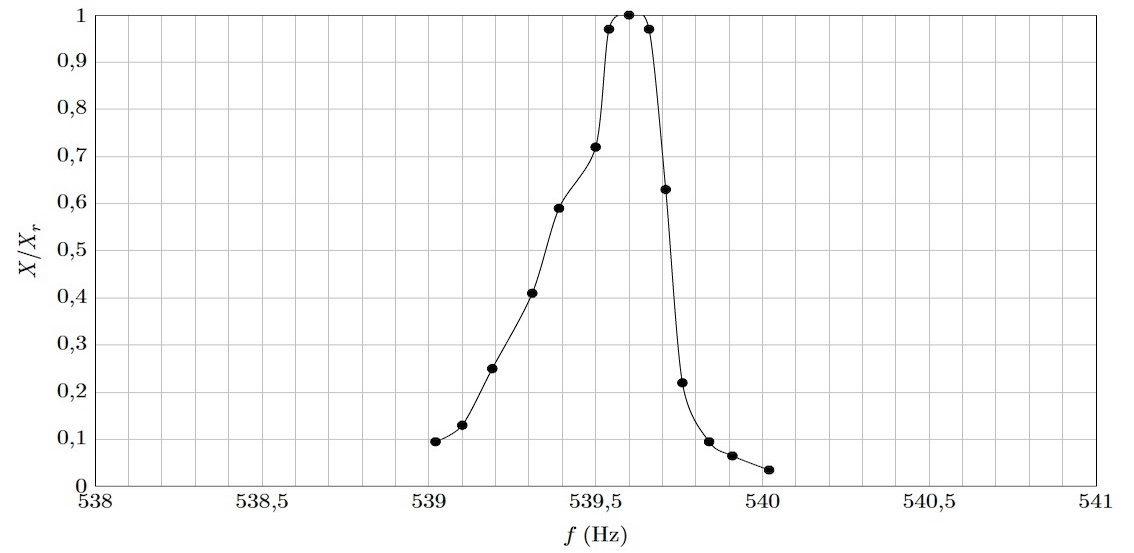
\includegraphics[width=.75\linewidth]{res_verre_7}
		\captionof{figure}{Amplitude relative en fonction de la fréquence.}
		\label{fig:bode_expe}
	\end{center}

}

\QR[7]{%
	Déterminer, à l'aide de la figure \ref{fig:bode_expe}, la pulsation propre
	$\w_0$ et le facteur de qualité $Q$ du verre dans son mode 1. Vous recopierez
	sommairement la figure sur votre copie pour faire apparaître votre
	construction graphique. Comparer avec les résultats de la première partie.
}{%
	~
	\vspace{-15pt}
	\smallbreak
	\begin{isd}[interior hidden]
		\begin{center}
			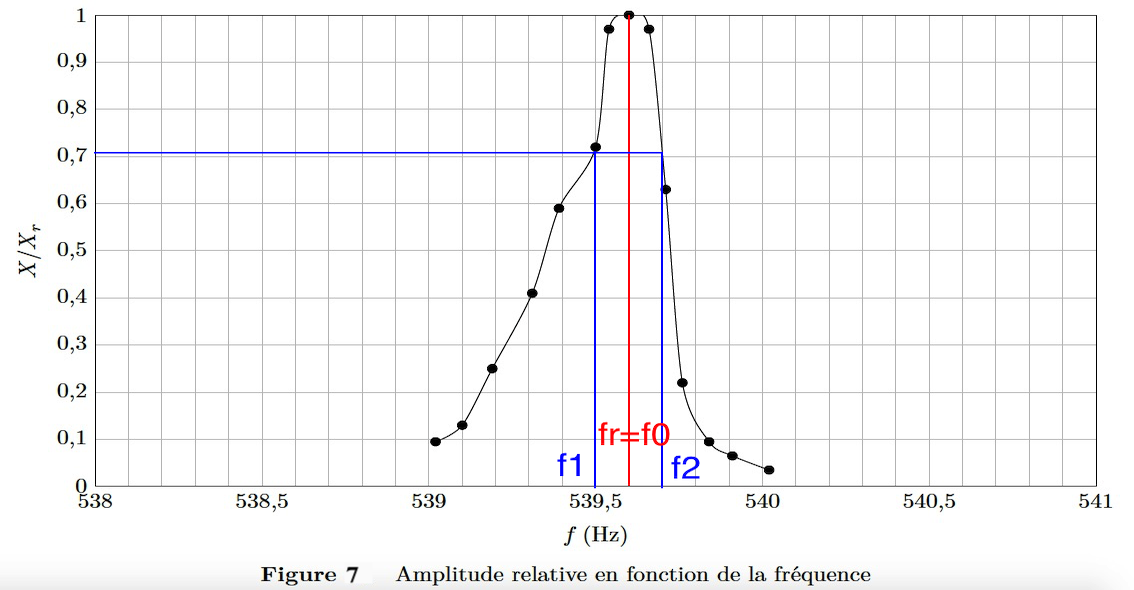
\includegraphics[width=\linewidth]{res_verre_7c}
			\captionof{figure}{\protect\pt{1}+\protect\pt{1}}
		\end{center}
		\tcblower
		On a vu précédemment que le système étudié possédait bien un facteur de
		qualité très élevé, on a donc $\w_r\approx \w_0$. On relève
		$f_r=f_0=\SI{539,6}{Hz}$ \pt{1}, soit \xul{$\w_0=\SI{3390}{rad.s^{-1}}$}.
		\smallbreak
		Les fréquences de coupures, telles que $X/X_r=\frac{1}{\sqrt{2}}\approx
			\num{0.71}$ \pt{1}, valent respectivement $f_1=\SI{539,5}{Hz}$ et
		$f_2=\SI{539,7}{Hz}$ \pt{1}
		\smallbreak
		On en déduit $Q = \dfrac{\w_0}{\w_2 - \w_1} = \dfrac{f_0}{f_2-f_1} =
			\num{2.7e3}$. \pt{1}
		\smallbreak
		On retrouve bien environ les mêmes valeurs que dans la première partie. \pt{1}
		La détermination de $\w_0$ est cependant plus précise au vu de l'échelle du
		graphique.
	\end{isd}
	\vspace{-15pt}
}

\QR[5]{%
	En musique, la gamme tempérée comporte 12 demi-tons (Do - Do$\sharp$ - Ré -
	Ré$\sharp$ - Mi - Fa - Fa$\sharp$ - Sol - Sol$\sharp$ - La - La$\sharp$ - Si).
	Pour passer d'une note à la note suivante, on multiplie sa fréquence par
	$2^{1/12}$. Sachant que le La3 se trouve à \SI{440}{Hz}, quelle note doit
	chanter la \textsc{Castafiore} pour briser le verre~? Chante-t-elle juste~?
}{%
	Pour briser le verre, il faut le mettre en résonance de sorte à ce qu'il vibre
	avec une amplitude telle que la déformation du matériau provoque sa rupture.
	\pt{1} Il faut donc l'exciter à la fréquence de \SI{539.6}{Hz}. \pt{1}
	\smallbreak
	Si on a la note La à \SI{440}{Hz}, alors les notes suivantes dans la gamme ont
	pour fréquences~: \pt{1} \SI{466}{Hz} (La$\sharp$) , \SI{494}{Hz} (si),
	\SI{523}{Hz} (do) et \SI{554}{Hz} (do$\sharp$).
	\smallbreak
	D'après la courbe, on voit qu'à \SI{554}{Hz}, la résonance est déjà passée.
	\pt{1} Il faut donc chanter à une fréquence intermédiaire entre celle du Do et
	du Do$\sharp$. En en conclut donc que la \textsc{Castafiore} chante faux
	lorsqu'elle brise le verre~! \pt{1}
}

\end{document}
